\chapter{Introduction}
\label{introchap}

The proposed dissertation research will ask how linguists should approach language documentation and description in order to achieve optimal results from machine learning. Machine learning can provide automated assistance but linguists must know how to make effective use of it. The proposed research will focus on effective integration of machine learning into the struggle to document and describe endangered language with speed and accuracy. It will look specifically at methods of interlinearization and inflectional paradigm induction.
%The proposed research focuses on effective integration for morphological annotation and analysis.

\begin{figure}[h]
\centering
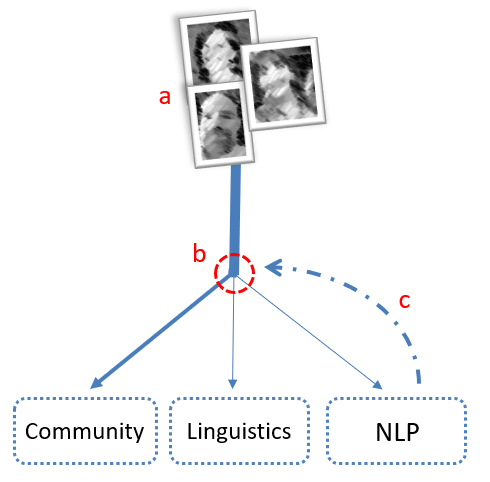
\includegraphics[width=7cm]{figs/Flowchart.PNG}
\caption[Language Data Production]{In language documentation and description, a team of linguists and native speakers (a) collaborate to document language data that benefits the community of speakers, linguistic sciences, and NLP development. However, a bottleneck of time-consuming annotation (b) makes keeps data largely inaccessible. The proposed research examines ways that linguists can address this by integrating machine learning (c).}
\label{fig:flowchart}
\end{figure}

\section{Background}

In the early 1990s it was suggested that linguistics might be the first academic discipline to preside over its own demise. As much as 90\% of the world’s 7,000 languages are predicted to become extinct by the end of the 21st century \cite{krauss_worlds_1992,krauss_keynote--mass_2007,campbell_new_2013}. Many languages will disappear without sufficient documented data to describe their structure and history. In response to this, linguists gave greater emphasis to documenting and describing endangered languages. Since the disquieting warning of language endangerment, documentary and descriptive activities have achieved impressive results. However, this work 
%including the process of annotating texts and analyzing morphological paradigms, 
must be increased and improved if it is to counteract the crisis of language endangerment. 
This will require better integration of computational methods into the process of language documentation and description. 

During that same time period, machine learning systems, capable of learning complex patterns in data, have gained tremendous success in natural language processing (NLP). Typically, state-of-the-art systems require hundreds of thousands, or even millions, of data instances (words, sounds, sentences, etc.) to achieve state-of-the-art results. Few languages have more than a couple of thousand tokens,
%, let alone much available data, 
so NLP research has been limited to handful of major languages, such as Chinese, Arabic, English and other European languages. None of these languages 
%demonstrate complicated morphology polysynthetic type, none are under-documented, none 
are endangered.\mans{The big data requirement is pretty specific to neural models.}

Thanks to the emphasis on documentary and descriptive fieldwork, our knowledge of the world's language is broadening beyond economically or politically powerful languages, but NLP has not responded as quickly. Fortunately, this seems to be changing. In recent years, NLP research in settings with limited data has burgeoned. This is evidenced, for instance, by the 2015-2019 DARPA-funded LORELEI project, motivated in part by the 2014 Haiti earthquake where disaster aid workers struggled to process social media posts in Haitian Creole.

Despite this growth, very few NLP systems have been integrated into the process of documenting and describing endangered languages. This may be due to the specific challenges presented by the dynamic, evolving nature of ongoing linguistic analysis and the inconsistencies that arise during the manual annotation. These challenges illustrate why documentary and descriptive linguists must adjust their methods
%their methods to the specifications of machine learning specifications 
in order to effectively benefit from machine learning.
%into language documentation and description. 

\section{Overview of Proposed Research}

Once language data has been analyzed and annotated it becomes usable for further scientific discovery in linguistics and NLP. After documented data is transcribed, it is annotated with basic linguistic analysis in a multi-step process called interlinearization. Narrowly defined, interlinearization comprises three tasks: 1) segmenting words into morphemes, 2) glossing each morpheme with its narrow lexical or grammatical translation, and 3) freely translating whole sentences into a language of wider communication to show how the morphemes combine to create meaning. The result is illustrated in (\ref{ex:IGTex}) with a transliterated Russian sentence. Interlinearization lays the foundation for other analysis and annotation, such as identifying morphological inflectional patterns.  
%Although textual data contains many repeated linguistic structures, it is only by 
%Interlinearizing all data uncovers rare and unique linguistic phenomena among the very common and frequently repeated structures. 

\begin{singlespace}
\pex<IGTex>   
\label{ex:IGTex}
\textbf{Text:} \hspace{14 mm} Vecherom \hspace{4.75 mm} ya \hspace{13 mm} pobejala \hspace{21 mm} v \hspace{2 mm} magazin \\
\textbf{Segmented:} \hspace{2 mm} vecher-om \hspace{4 mm} ya \hspace{13 mm} pobeja-la \hspace{20 mm} v \hspace{2 mm} magazin \\
\textbf{Glossed:} \hspace{8.5 mm} evening-\textsc{ins} \hspace{1 mm} 1.\textsc{sg.nom} \hspace{1 mm} run-\textsc{pfv.pst.sg.fem} \hspace{1 mm} in \hspace{1 mm} store.\textsc{acc} \\
\textbf{Translation:} \hspace{1 mm} `In the evening I ran to the store.' \\
\xe
\end{singlespace}


The proposed dissertation is motivated by a “yawning gap” \cite{seifart_language_2018} between the amount of documented data deposited in language archives and the portion of the data that is usable for research. This gap is caused by what has been described as an annotation bottleneck, illustrated in Figure \ref{fig:bottleneck}. The bottleneck is created by currently accepted but tedious and time-consuming methods that are done primarily by hand from start to finish \cite{simons_worlds_2013,holton_developing_2017}. 
%The process is labor- and time-intensive. Manual annotation is subject to human error, with many mistakes and inconsistencies due not to the difficulty of the task, but to its repetitive and monotonous nature.
Budget constraints often mean that large portions of the data produced by field projects are left unannotated. They remain untapped resources for science and human language technology that would benefit the language communities. 

The proposed research asks: \emph{How should the integration of machine learning into language documentation and description influence accepted methods of annotation% during basic linguistic analysis
?} It will use machine learning and corpora from six endangered or under-documented languages. It will 
%address the annotation bottleneck by examining 
examine how current methods affect machine learning performance and the potential to incorporate more automated assistance. This will be done with three studies:

\begin{enumerate}
\item{} \textbf{Automating Segmentation and Glossing:} How do choices made during interlinearization (i.e. surface versus canonical segmentation, in/consistent morpheme boundaries, lack/presence of part of speech tags) affect machine learning results on morpheme segmentation and glossing? 
     \begin{itemize}
        \item To what extent do these choice affect the performance of a neural Transformer model compared to a Conditional Random Fields model? 
        \item To what extent do they make a pipeline approach preferable to joint learning of morpheme boundaries and glosses?
    \end{itemize}
\item{} \textbf{Balance of Interlinearization Tasks:} When faced with limited time, how does integration of machine learning dictate the priorities of completing different interlinear lines? 
%segmentation and glossing over free translation? 
    \begin{itemize}
        \item{} What ratio of completed lines achieves optimal machine learning performance on all interlinear lines?
        \item{} To what extent does completion of other interlinear lines affect the results on any one line? I.e.  Does leveraging glosses improve machine translation? Can information extracted from other lines of interlinear glossed texts improve segmentation and glossing?  
    \end{itemize}
\item{} \textbf{Morphological Description:} To what extent can manually interlinearized texts be utilized for computational induction of morphological inflection patterns? 
    \begin{itemize}
    \item{} Does manual cleaning of the data improve performance?
    \item{} Are part of speech tags necessary for this task?
    \end{itemize}
\end{enumerate}

The first part of the proposed dissertation research will discover what choices by annotators and what machine learning models are mostly likely to speed and improve segmentation and glossing of under-documented languages. It will train three machine learning systems to segment and gloss in four languages. These languages have been segmented with two strategies that will be used to train different models. The results from each will be compared across the three systems.  

The second part of the proposed research will find the balance of completed tasks that give optimal results in both automated segmentation/glossing and machine translation. It will use various ratios of completion and find the optimal ratio. It will data from two languages which have relatively large amount of interlinear texts. Two machine learning models will be trained to segment and gloss and two to translate. One model from each will be trained on input that leverages information from other completed tasks. The relative differences in results for segmentation/glossing and translation will be compared.

The third part proposes new computational methodology for assisting the analysis and description of morphological inflection patterns. It will learn inflectional paradigms from the interlinear texts in six languages. A machine learning model will be trained to generate inflected forms not previously seen by the model. One system will integrate manual work and use the model as automated assistance. Another system will use an automated process. The results of the two will be compared.

\section{Expected Results and Implications}

\begin{figure}[h!]
    \centering
    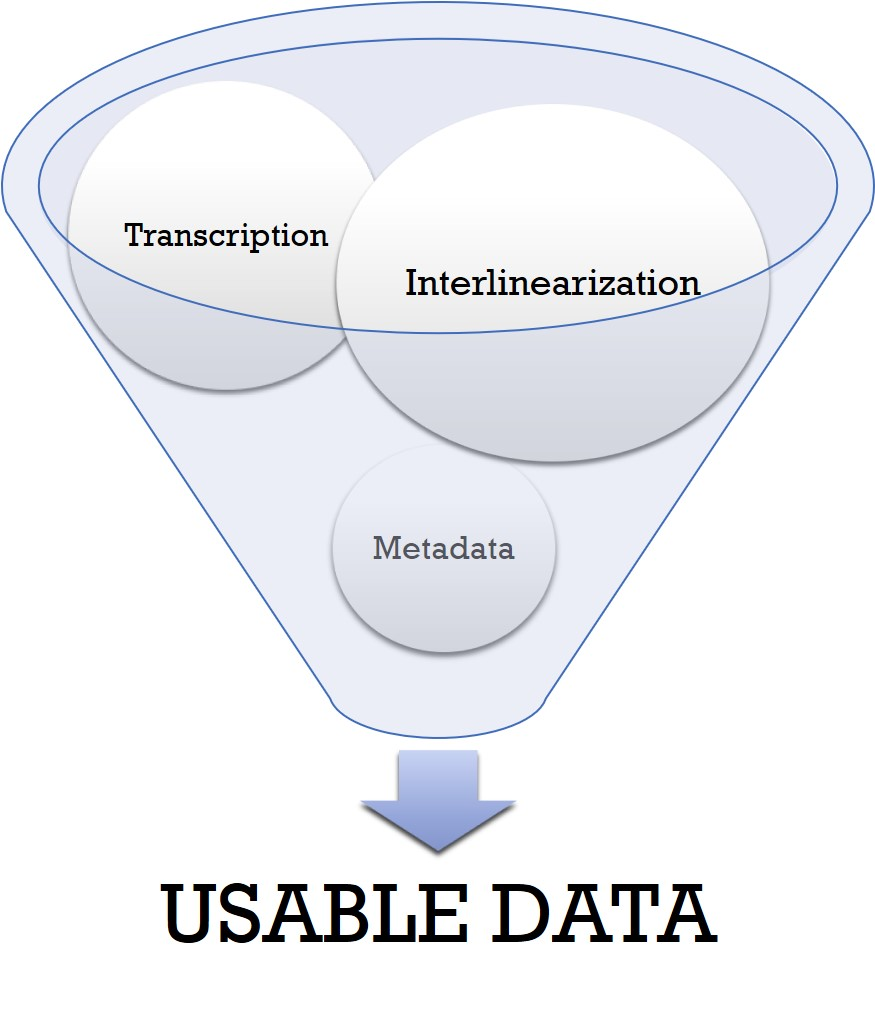
\includegraphics[width=7cm]{figs/AnnotationFunnel.jpg}
    \caption[Annotation Bottleneck]{Annotation bottleneck in language documentation and description.}
    \label{fig:bottleneck}
\end{figure}


The proposed research will support more effective integration of computational methods in order to reduce the bottleneck caused by current time-consuming manual methods to produce morpheme segmentation, glossing, free translation, and first-pass hypotheses of morphological inflectional paradigms. It will unite the efforts of linguistics and NLP by training machine learning on linguistic field data and examining how linguistic field methods might affect the results. Since this research will be performed on “real live” field data---sometimes the only annotated data available for a language---it may uncover unforeseen challenges for NLP in low-resource settings that is normally trained on curated published data. 

The contribution of this dissertation research is four-fold. First, it will increase annotated data in NumLG endangered and low-resource languages whose manually annotated data is currently limited to 2K-100K words.  These languages represent a broad range of linguistic structures and language families. They are spoken by communities across five continents, but the amount of published linguistic resources for all is quite low. Increasing annotated data allows more thorough testing of linguistic theories and computational models, which contribute to our understanding of human language and the performance of machine learning algorithms in low-resource settings. 

Second, it will demonstrate how machine learning can be applied to specific sub-tasks of the documentary and descriptive pipeline to produce new annotated data more quickly and accurately than current manual methods. It will do this by constructing a pipeline of machine learning systems.

Third, the proposed dissertation will demonstrate the potential for machine learning to assist in linguistic analysis and language description by leveraging interlinearized glossed texts as training data. Specifically, it will use neural machine learning to learn inflectional patterns in six languages.\mans{``neural machine learning'' is perhaps a little too loose: neural networks might be better.} This is a step towards providing linguists with machine learning assistance when building a hypothesis of morphological inflectional paradigms in a language.

Fourth, the proposed research will establish not only that new computational methods can be successfully integrated into language documentation and description, but how integration of computational methods may impact commonly accepted practices in linguistics field methods. A main theme of the proposed research is that machine learning systems can take advantage of the typical output from documentary and descriptive field work. This dissertation will analyze the characteristics of that output which may affect the performance of machine learning systems trained on it. 

\section{Organization of Prospectus}

This Prospectus describes the author's planned dissertation research towards the goal of integrating machine learning into language documentation and description. Chapter \ref{chap:litreview} looks at the issues in previous research that is related to the proposed research. Chapter \ref{chap:datamodels} describes the data and the computational models that will be used in the research. Chapter \ref{chap:body} outlines the experiments that will be conducted and the results of pilot studies that have already been conducted. The Prospectus concludes with a timeline for the dissertation work and a discussion of the potential impact of this work.

